\begin{abstract}
Parallel code is notorious for its difficulties in writing, verification and maintenance. However, it is of increasing importance, following the end of Moore's law. Modern programmers are expected to utilize the power of multi-core CPUs and face the challenges brought by parallel programs.

This project builds an embedded framework in Haskell to generate parallel code. Combining the power of multiparty session types with parallel computation, it creates a session typed monadic language as the middle layer and use Arrows, a general interface to computation as an abstraction layer on top of the language. With the help of the Arrow interface, we convert the data flow of the computation to communication and generate parallel code according to the communication pattern between participants involved in the computation. Thanks to the addition of session types, not only the generated code is guaranteed to be deadlock-free, but also we gain a set of local types so that it is possible to reason about the communication structure of the parallel computation.

In order to show the framework is as expressive as usual programming languages, we write a few common parallel computation patterns and three algorithms to benchmark using our framework. It demonstrates that users can express computation similar to traditional sequential code and gain a high-performance parallel code in low-level target languages such as C for free and the use case of the framework is not limited to a standalone tool for parallel computation; we show the framework can act as a code generation backend for other data-flow based high-level parallel languages with an example. Benchmarks show the generated code can have up to 12X speedup on certain input sizes on a 32-core machine.
\end{abstract}


\renewcommand{\abstractname}{Acknowledgements}
\begin{abstract}
TBD
\end{abstract}

\tableofcontents
% \listoffigures
% \listoftables
\chapter{Introduction} \label{chap:intro}

\section{Motivation} \label{i:m}
Writing parallel software is not a trivial task. Parallel code is hard to write because it is usually done in low-level languages with verbose and non-idiomatic decorations, hard to debug because machines, where code is written, are usually different from machines where code is intended to run and hard to maintain and reuse. This is because even though the underlying algorithms are not changed, multiple version of parallel code is needed to tackle various platform and evolution of architectures.

There are many on-going pieces of research aimed at helping programmers to write correct parallel programs smoothly. A common approach is to develop a high-level language and compile programs in this language to parallel code. There are many high-level frameworks for parallel programming (\eg algorithmic skeletons\cite{coleAlgorithmicSkeletonsStructured}, domain-specific languages for parallelism\cite{brownHeterogeneousParallelFramework2011} or the famous MapReduce parallel model\cite{liMapReduceParallelProgramming2016}). An example is to use arrow terms (\secref{b:arrows}) to describe data flow implicitly and hence generate parallel code \cite{braunArrowsParallelComputation2018}.

The workflow of writing parallel code has evolved from writing it directly in the target platform to writing software in a high-level language designed for parallel computation and then compiling to the target platform. In this project, we present a method to improve the backend of parallel code generation by introducing a monadic domain-specific language: SPar to act as a bridge between high-level and target low-level parallel languages.

This specific language needs to be general enough so that it supports multiple high-level parallel programming frameworks. It can be used to generate different parallel code such as Message Passing Interface (MPI) and Cuda. Moreover, we developed a simulator to aid debugging parallel programs.

% With the help of this intermediate languages, the implementation complexity is reduced from $O(M \times N)$, where each of the M high-level languages needs to implement N compilers to generate parallel code in N different platforms, to $O(M + N)$, where each compiler of a high-level language implements a translation rule to the intermediate language which implements one compiler and N backend to generate different target languages.

Our framework couples with multiparty session type (MPST) \cite{coppoGentleIntroductionMultiparty2015}. It is done by inferring session types for computation of each participant. We can take advantages of the collection of local types to enable aggressive optimization but ensuring code correctness and meaningful static analysis; \eg cost modelling for parallel programming according to properties of MPST.
\section{Contributions} 
\begin{figure}[ht]
    \centering
    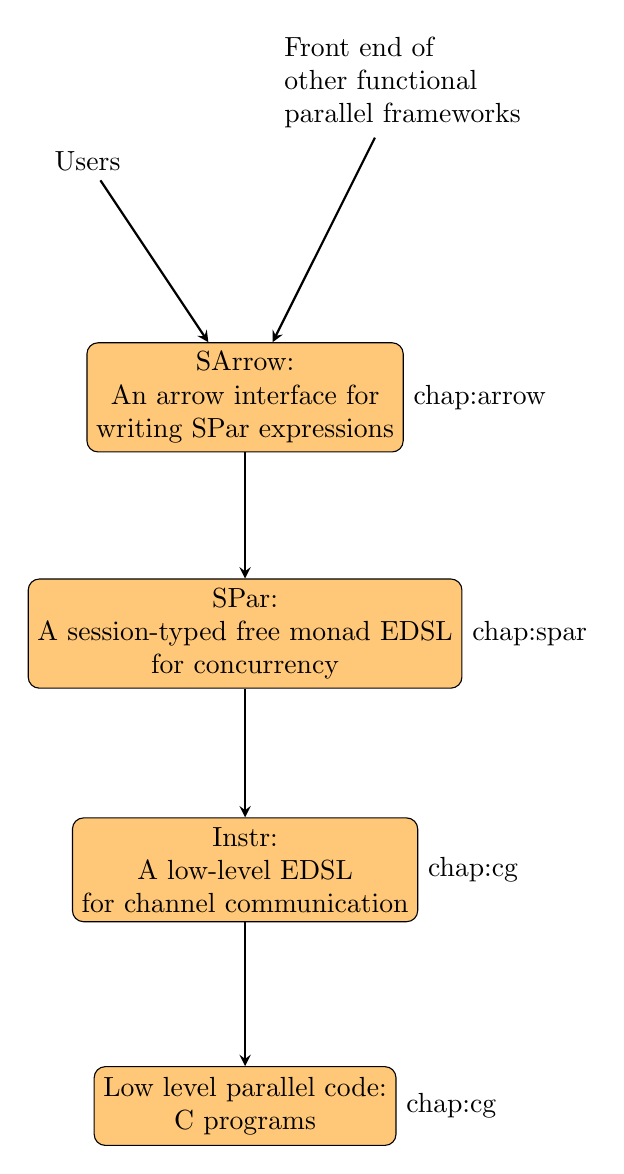
\begin{tikzpicture}[xscale=.5]
    \tikzstyle{proc}  = [rectangle, rounded corners, minimum width=2cm, minimum height=1cm,text centered, draw=black, fill={rgb:orange,1;yellow,2;pink,5}, align=center]
    \tikzstyle{proc1} = [circle,  minimum width=2cm, minimum height=5cm,text centered, draw=black] 
    \tikzstyle{arrow} = [thick,->,>=stealth]
    \node (a) [proc, label=right:\charef{chap:arrow}] at (0, 3)  {SArrow: \\ An arrow interface for \\ writing SPar expressions};
    \node (b) [proc, label=right:\charef{chap:spar}] at (0, 0)  {SPar: \\  A session-typed free monad EDSL \\ for concurrency};
    \node (c) [proc, label=right:\charef{chap:cg}] at (0, -3) {Instr: \\ A low-level EDSL \\ for channel  communication};
    \node (f) [proc, label=right:\charef{chap:cg}] at (0, -6) {Low level parallel code: \\ C programs};
    % \node (f) [proc, label=right:\charef{chap:cg}] at (0, -6) {Instr: \\ A low-level EDSL \\ for channel  communication};
    \node (d)  at (-4, 6) {Users};
    \node (e) [align=left] at (4, 7) {Front end of \\ other functional  \\ parallel frameworks};
    \draw[arrow] (a) to (b);
    \draw[arrow] (b) to (c);
    \draw[arrow] (d) to (a);
    \draw[arrow] (e) to (a);
    \draw[arrow] (c) to (f);
    \end{tikzpicture}
    \caption{Visualization of the workflow}
    \label{intro:fig:workflow}
\end{figure}
The result of project is an embedded high-level framework in Haskell that is capable of generating low-level parallel code. The major contributions are:
\begin{enumerate}
    \item \textbf{Session-typed intermediate language. } We create an intermediate embedded domain specific language (EDSL): \textbf{SPar}: a session typed free monad EDSL for message passing concurrency. SPar is built using free monad technique, and it contains primitive operations for channel communication as well as its representation of computation. This language can be typed by local types, and hence, we can apply multiple results from the multiparty session types to our framework, especially in terms of safety of generated code and reasoning of communication patterns.
    \item \textbf{Intuitive user interface. } One innovation of this project is that we apply the Arrow interface for users to express parallel computations. Arrow is a general interface for computations (see in \secref{b:arrows}). We call our interface \textbf{SArrow}: an arrow interface for writing SPar expressions. It is an abstraction layer on top of SPar, which hides communication primitives from users so that users can express parallel algorithms similar to what they would write for sequential programs.
    \item \textbf{Multiple backends. } We create a backend to generate parallel C code from SPar expressions. The core of the backend is \textbf{Instr:} a low-level EDSL for channel communication as well as operations on variables and resources management. It is independent of target languages. This means that we can support multiple target languages with ease without re-implementing multiple backends. In addition to the code generation backend, we implement an interpreter backend in Haskell for experimenting and fast verification.
    \item \textbf{Evaluations. } Finally, we show the expressive power of the framework by implementing several common computation patterns and three algorithms using our interface. We evaluate the performance of the generated code from the algorithms on high-performance computers as well as PCs. 
\end{enumerate}
The \figref{intro:fig:workflow} summaries the workflow of the framework visually. The main principle supporting the framework is that \textbf{we convert data flow into communication and from the communication pattern, we gain parallel code}. The results of expressing computation in the framework are 1) compilation to efficient deadlock-free low-level parallel programs and 2) a set of local types to reason the structure of the parallel computation.

At the end of the project, we have discovered two use case of the framework. The primary application is a stand-alone tool to generate parallel C code from programs written in Haskell, and another is a backend for other data-flow based parallel frameworks. 

\section{Report outline}

\charef{chap:b} gives an overview of the background and related research. We present the syntax and semantics of SPar in \charef{chap:spar} followed by \charef{chap:impl} introducing the implementation aspect of SPar, like session typing and developing the interpreter. \charef{chap:arrow} demonstrates the Arrow interface with examples of parallel patterns formed by the interface and justification of the interface satisfying the arrow laws. The discussion about some implementation specific issues like role allocation is also contained in \charef{chap:arrow}. In \charef{chap:cg}, we show the code generation backend and discuss our solutions to challenges when compiling to C, i.e. the problem of representing polymorphic algebraic data structures in C. \charef{chap:eval} explains our benchmark and shows the performance of the generated code. This chapter can also be regarded as a tutorial on how to use the framework. Finally, we conclude with potential future improvements and remarks on this project. We also include the generated C code in the appendix for the curious readers.